%---------------------------------------------------------------------
%
%                          Cap�tulo 2
%
%---------------------------------------------------------------------


\chapter*{%
\href{http://www.sciencedirect.com/science/article/pii/S2212968515000112}{%
Proteopathogen2: A database and web tool to store and display  proteomics identification results in the mzIdentML standard%
}%
}
\addcontentsline{toc}{chapter}{Proteopathogen2: A database and web tool to store and display  proteomics identification results in the mzIdentML standard}
%\fancyhf{} % clear all header and footer fields

%Ojo, solo para la versi�n B5
\addtocontents{lof}{\protect\newpage} %Ojo, solo para la versi�n B5



\addcontentsline{lof}{chapter}{Proteopathogen2: A database and web tool to store and display  proteomics identification results in the mzIdentML standard}
\addcontentsline{lot}{chapter}{Proteopathogen2: A database and web tool to store and display  proteomics identification results in the mzIdentML standard}



%\renewcommand{\headrulewidth}{0pt}
\cabeceraEspecial{Proteopathogen2, adapted to mzIdentML}

\subsubsection*{Vital Vialas, Concha Gil}
\subsubsection*{EuPA Open Proteomics 2015, 8, 22-27}

\bigskip
\hfill
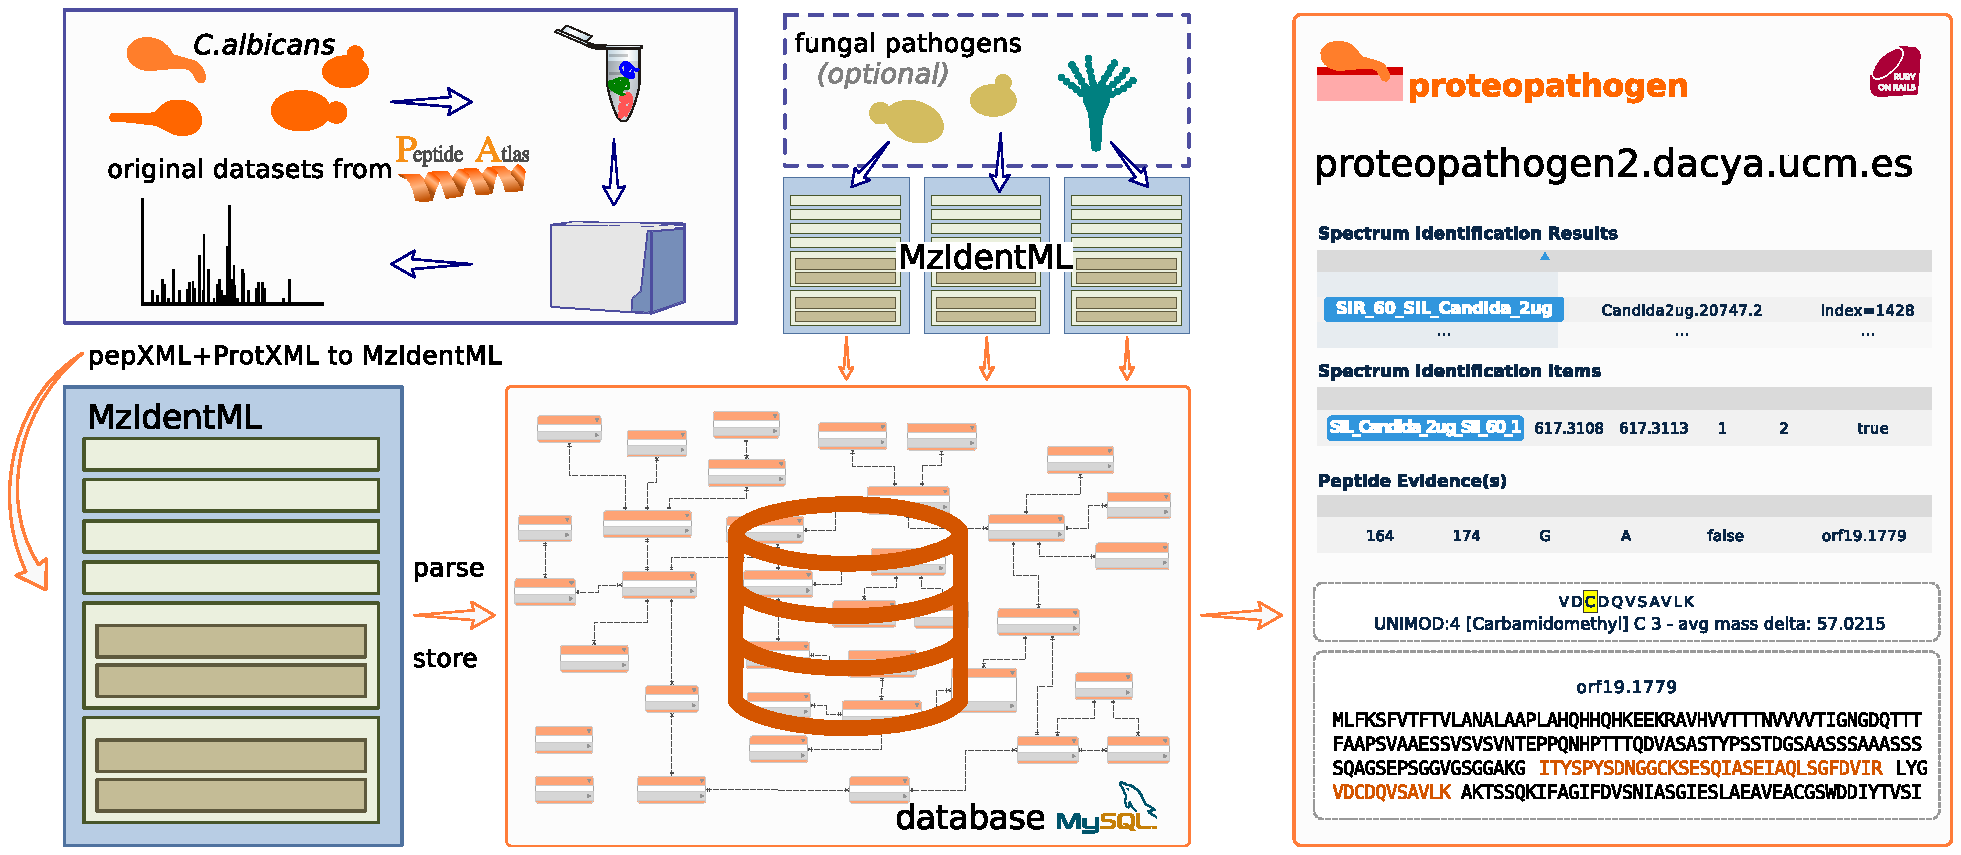
\includegraphics[width=1\textwidth]{Imagenes/Vectorial/graphical_abstract_proteopathogen2}



\newpage


%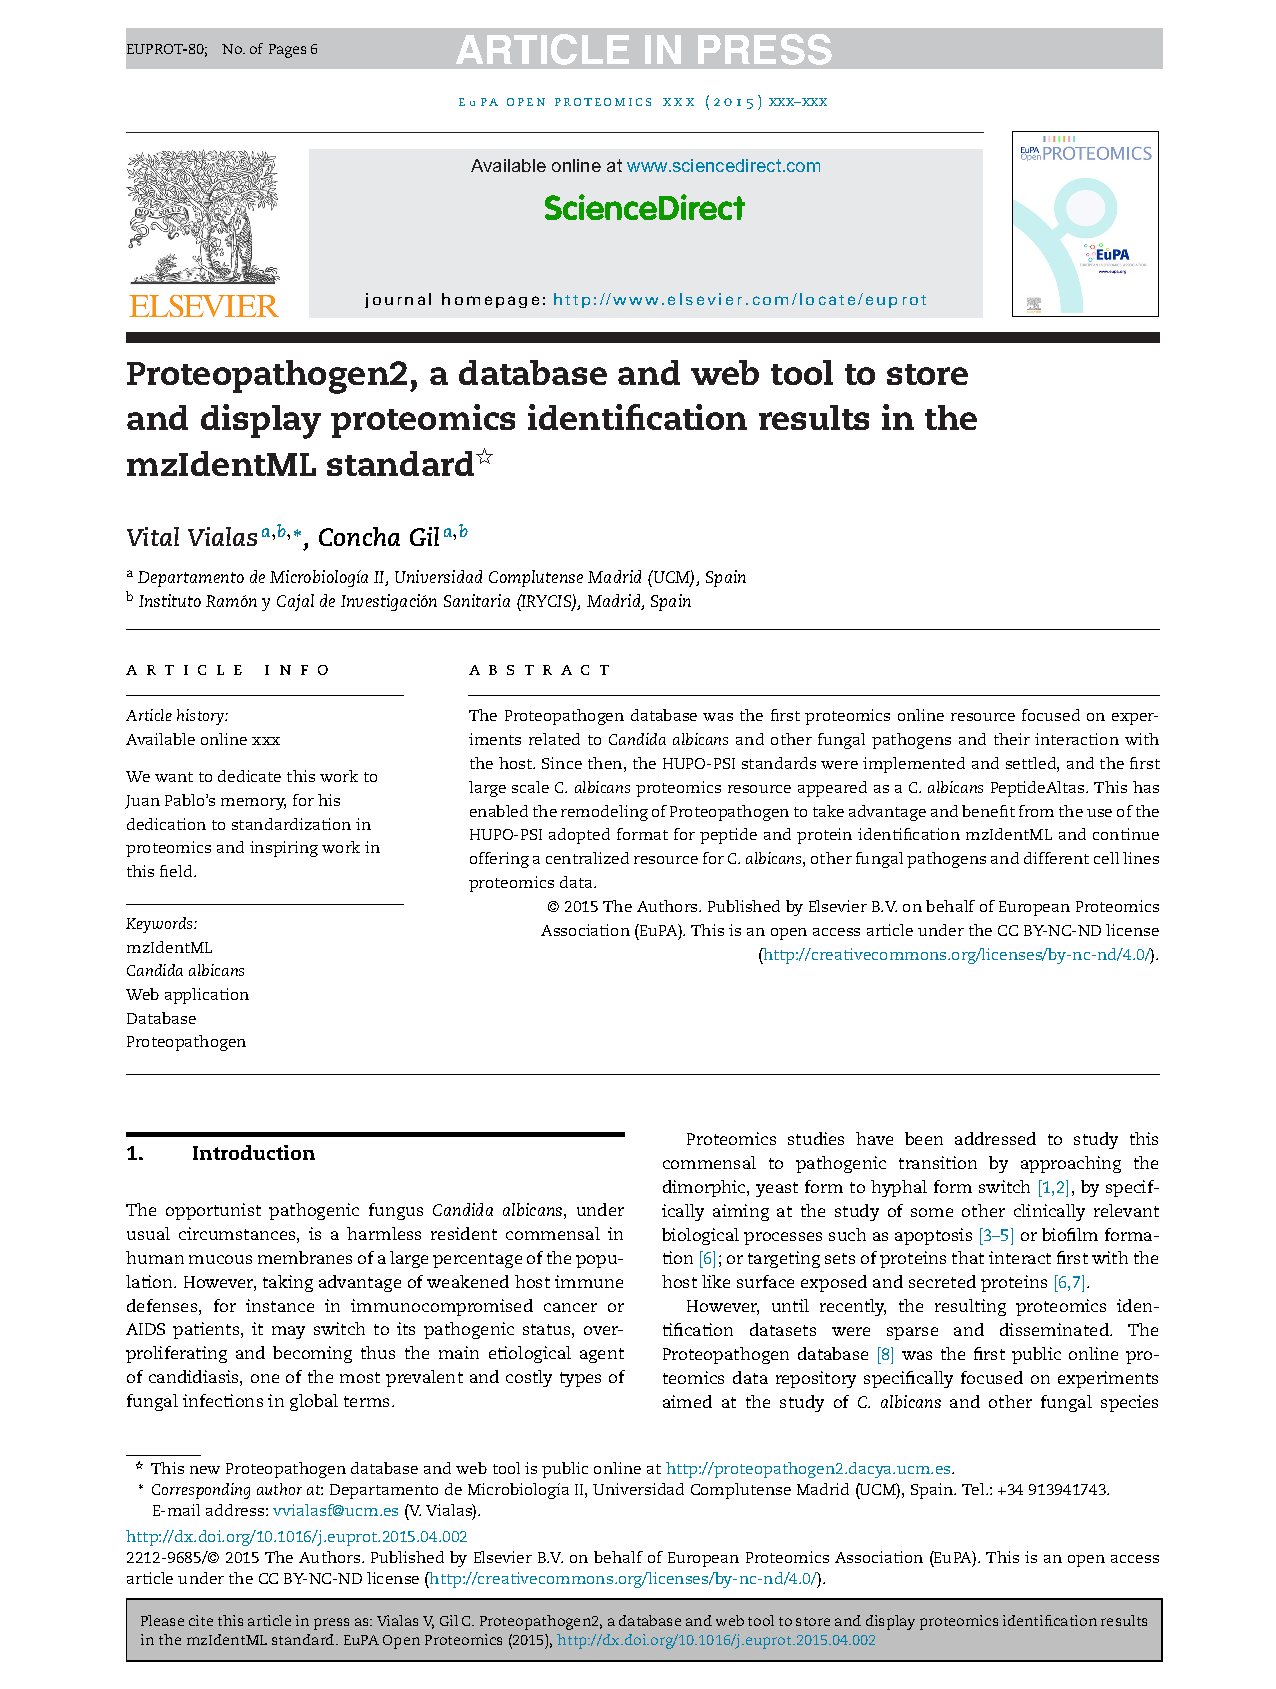
\includepdf[pages=-,pagecommand={}]{Proteopathogen/Vialas_2015_Proteopathogen2_EupaOpen.pdf}


\chapter*{Abstract}
The Proteopathogen database was the first proteomics online resource 
focused on experiments related to \textit{Candida albicans}
 and other fungal pathogens and their interaction with the host. 
 Since then, the HUPO-PSI standards were implemented and settled, and 
 the first large scale \textit{\mbox{C. albicans}} proteomics resource appeared 
 as a \textit{\mbox{C. albicans}} PeptideAltas. This has enabled the remodeling
 of Proteopathogen to take advantage and benefit from the use of the 
 HUPO-PSI adopted format for peptide and protein identification mzIdentML 
 and continue offering a centralized resource for \textit{\mbox{C. albicans}}, 
 other fungal pathogens and different cell lines proteomics data.

\newpage{}

\section*{Introduction}
\addcontentsline{toc}{section}{Introduction}

The opportunist pathogenic fungus \textit{Candida albicans}, under
usual circumstances, is a harmless resident commensal in
human mucous membranes of a large percentage of the population.
However, taking advantage of weakened host immune
defenses, for instance in immunocompromised cancer or
AIDS patients, it may switch to its pathogenic status, over-
proliferating and becoming thus the main etiological agent
of candidiasis, one of the most prevalent and costly types of
fungal infections in global terms.

Proteomics studies have been addressed to study this
commensal to pathogenic transition by approaching the
dimorphic, yeast form to hyphal form switch \citep{Monteoliva2010,Gow2011},
by specifically aiming at the study of some other clinically relevant
biological processes such as apoptosis \citep{Madeo2004, Fernandez-Arenas2007, Ramsdale2008} 
or biofilm formation \citep{Vialas2012};
or targeting sets of proteins that interact first with the
host like surface exposed and secreted proteins \citep{Vialas2012, Gil-Bona2015a}.

However, until recently, the resulting proteomics identification
 datasets were sparse and disseminated. The
Proteopathogen database \citep{Vialas2009b} was the first public online 
proteomics data repository specifically focused on experiments
aimed at the study of \textit{\mbox{C. albicans}} and other fungal species
pathogenic traits. Since no standard format for peptide and
protein identification results was available, Proteopathogen
was developed to compile and display identification lists in
different tabulated text formats depending on the software
used to generate and process the results.

At that time, the HUPO - Proteomics Standards Initiative
(PSI) already had a trajectory striving to highlight the importance 
of standardization and providing formats that would
comply with MIAPE (Minimum Information About a Proteomics
Experiment) guidelines as reviewed in ref \citep{Martinez-Bartolome2014}. 
Some \textit{de facto}
standard formats existed like mzXML and pepXML \citep{Deutsch2012}, but the
advent, years later, of the HUPO-PSI approved formats for mass
spectrometry output data \citep{Martens2011} and for identification results \citep{Jones2012}
among others, surfaced the efforts and claims by the community to finally
 adopt formats to facilitate data comparison,
exchange and verification. This also inspired and boosted the
development of an assortment of format conversion tools and
libraries \citep{Chambers2012, Griss2012} and stand-alone software for visualization of
the content of the files in standard formats \citep{Ghali2013} but, most
importantly for the purpose of this work, enabled the possibility
 for Proteopathogen to benefit from the mzIdentML adopted
standard for identification results, incorporating it as the input
data format and using it as inspiration for information display.

More recently, the most comprehensive, up to the current date, 
online \textit{\mbox{C. albicans}} proteomics data repository was
developed and integrated in PeptideAtlas \citep{Vialas2013}. These publicly
available \textit{\mbox{C. albicans}} results have been used to establish a new
version of Proteopathogen with a solid foundation.

In this background, we present here a revisited Proteopathogen
 database and web based tool adapted to read and
display peptide and protein identification data based upon
the mzIdentML format. It is the first online database specifically
 developed to map and store the contents of files in
mzIdentML, it has been initially populated with the \textit{\mbox{C. albicans}}
PeptideAtlas identification results and it is publicly accessible
at \href{http://proteopathogen2.dacya.ucm.es}{http://proteopathogen2.dacya.ucm.es}

\phantomsection{}
\section*{Materials and methods}
\addcontentsline{toc}{section}{Materials and methods}

The original identification result files were obtained from
PeptideAtlas repository datasets 
\href{ftp://ftp.peptideatlas.org/pub/PeptideAtlas/Repository/PAe001976/}{PAe001976},
\href{ftp://ftp.peptideatlas.org/pub/PeptideAtlas/Repository/PAe001977/}{PAe001977},
\href{ftp://ftp.peptideatlas.org/pub/PeptideAtlas/Repository/PAe001978/}{PAe001978}, 
\href{ftp://ftp.peptideatlas.org/pub/PeptideAtlas/Repository/PAe001979/}{PAe001979}, 
\href{ftp://ftp.peptideatlas.org/pub/PeptideAtlas/Repository/PAe001980/}{PAe001980}, 
\href{ftp://ftp.peptideatlas.org/pub/PeptideAtlas/Repository/PAe001981/}{PAe001981}, 
\href{ftp://ftp.peptideatlas.org/pub/PeptideAtlas/Repository/PAe001982/}{PAe001982},
\href{ftp://ftp.peptideatlas.org/pub/PeptideAtlas/Repository/PAe001983/}{PAe001983}, 
\href{ftp://ftp.peptideatlas.org/pub/PeptideAtlas/Repository/PAe001984/}{PAe001984}, 
\href{ftp://ftp.peptideatlas.org/pub/PeptideAtlas/Repository/PAe001985/}{PAe001985}, 
\href{ftp://ftp.peptideatlas.org/pub/PeptideAtlas/Repository/PAe001986/}{PAe001986}, 
\href{ftp://ftp.peptideatlas.org/pub/PeptideAtlas/Repository/PAe001987/}{PAe001987},
\href{ftp://ftp.peptideatlas.org/pub/PeptideAtlas/Repository/PAe001988/}{PAe001988}, 
\href{ftp://ftp.peptideatlas.org/pub/PeptideAtlas/Repository/PAe001989/}{PAe001989}, 
\newline
\href{ftp://ftp.peptideatlas.org/pub/PeptideAtlas/Repository/PAe002110/}{PAe002110}, and 
\href{ftp://ftp.peptideatlas.org/pub/PeptideAtlas/Repository/PAe002111/}{PAe002111}.

As described in Ref. \citep{Vialas2013} the data sets come from a range
of experiments including yeast to hypha transition assays,
membrane protein extractions and a set of phosphoprotein
enrichment approaches. In all cases, cells from the clinical isolates
 SC5314 were grown in YPD medium. For obtaining cells
in hyphal form, either heat-inactivated fetal bovine serum or
Lee medium pH 6.7 was used. As for the mass spectrometry,
spectra were acquired in different set ups and platforms in a
data-dependent manner. A summary of the experiments set
ups and conditions is shown in Table 1.

\begin{table}[t]
\caption*{Table 1. Summary of experiments, MS output files, instrument and PeptideAtlas datasets.}
\renewcommand{\arraystretch}{2}
\footnotesize
\centering

\begin{tabular}{p{3cm} cp{2cm} p{2cm} p{2cm} }

\hline
Type of dataset & Number of \newline{} MS output files & Instrument & PeptideAtlas \newline{} datasets \\
\hline

\textit{Candida albicans} culture with SILAC labelling, digested protein extracts enriched in \newline phosphopeptides IMAC/TiO2 & 57 & Orbitrap XL, \newline{} Orbitrap Velos &
\href{ftp://ftp.peptideatlas.org/pub/PeptideAtlas/Repository/PAe001976/}{PAe001976},
\href{ftp://ftp.peptideatlas.org/pub/PeptideAtlas/Repository/PAe001977/}{PAe001977},
\href{ftp://ftp.peptideatlas.org/pub/PeptideAtlas/Repository/PAe001978/}{PAe001978}, 
\href{ftp://ftp.peptideatlas.org/pub/PeptideAtlas/Repository/PAe001979/}{PAe001979}, 
\href{ftp://ftp.peptideatlas.org/pub/PeptideAtlas/Repository/PAe001980/}{PAe001980}, 
\href{ftp://ftp.peptideatlas.org/pub/PeptideAtlas/Repository/PAe001984/}{PAe001984}, 
\href{ftp://ftp.peptideatlas.org/pub/PeptideAtlas/Repository/PAe001985/}{PAe001985}, 
\href{ftp://ftp.peptideatlas.org/pub/PeptideAtlas/Repository/PAe001986/}{PAe001986}, 
\href{ftp://ftp.peptideatlas.org/pub/PeptideAtlas/Repository/PAe001987/}{PAe001987},
\href{ftp://ftp.peptideatlas.org/pub/PeptideAtlas/Repository/PAe001988/}{PAe001988}, 
\href{ftp://ftp.peptideatlas.org/pub/PeptideAtlas/Repository/PAe001989/}{PAe001989} \\

\textit{Candida albicans} total protein extract, 2 Triple-TOF runs, 2ug and 4ug & 2 & Triple-TOF & 
\href{ftp://ftp.peptideatlas.org/pub/PeptideAtlas/Repository/PAe001983/}{PAe001983}  \\

Hyphal form and yeast form total protein extracts & 8 & Orbitrap Velos &
\href{ftp://ftp.peptideatlas.org/pub/PeptideAtlas/Repository/PAe002110/}{PAe002110}, 
\href{ftp://ftp.peptideatlas.org/pub/PeptideAtlas/Repository/PAe002111/}{PAe002111}\\

LTQ membrane proteins \newline \citep{Cabezon2009} & 3 & LTQ &  
\href{ftp://ftp.peptideatlas.org/pub/PeptideAtlas/Repository/PAe001981/}{PAe001981}\\

LTQ proteins from acidic subproteome \citep{Monteoliva2010} & 8 & LTQ & 
\href{ftp://ftp.peptideatlas.org/pub/PeptideAtlas/Repository/PAe001982/}{PAe001982}\\

\end{tabular}
\end{table}
\addcontentsline{lot}{table}{Table 1}


Consistently with the PeptideAtlas project principles, the
MS output files were processed through the Trans Proteomic
Pipeline. The steps involved, first, sequence database searching
 using X! Tandem with k-score \citep{MacLean2006} and a custom sequence
database obtained from Candida Genome Database \citep{Costanzo2006a} with
appended decoy counterparts and common contaminants for
peptide-to-spectrum matching and FDR assessment. Then
the post-processing validation tools PeptideProphet \citep{Choi2008}, 
ProteinProphet \citep{Nesvizhskii2003}
and iProphet \citep{Shteynberg2011} provided filtered lists of peptides
and proteins with high probabilities. And finally FDR was computed for
 different probability thresholds.

Each of the PeptideAtlas repository datasets consists on
the MS output spectra files and a set of pepXML and protXML
files with lists of high confidence peptide and proteins respectively. 
These were combined, independently for each dataset,
by means of a custom script written in the Ruby scripting language
 (available in supplemental data) to create mzIdentML
files (mzIdentML version 1.1.0) with the merged information.
In order to check the files were generated correctly and ensure
data quality they were all validated (semantic and MIAPE-
compliant validation) with mzidValidator \citep{Ghali2013}.

A completely new MySQL relational database was implemented \textit{ad hoc}
 to map elements in the mzIdentML files as
depicted in Fig. 1 (schema available in supplemental data).
Then, using the Ruby scripting language (version 2.0.0) and
the Rails web application development framework (version
4.0.0) a script was created to parse the data in the mzIdentML
files, store the relevant elements in the corresponding tables
(available in supplemental data) and eventually create the web
application to display the data.



\phantomsection{}
\section*{Results and discussion}
\addcontentsline{toc}{section}{Results and discussion}


A total number of sixteen mzIdentML files, corresponding to
each of the PeptideAtlas repository datasets, grouped into
five different experiments were compiled and used to initially
 populate the Proteopathogen database. These account
for approximately 22,000 distinct peptides and 2600 different proteins
 that can be queried and viewed through the web
interface.

\begin{figure}[t]
\begin{center}
 \includegraphics[width=0.70\textwidth]%
				 {Imagenes/Vectorial/proteopathogen2_figure1}
\caption*{Figure 1. mzIdentML to database mapping. The MySQL schema was 
specifically designed to accommodate elements from the mzIdentML format.
Figure shows the one-to-many relationship between the 
<SpectrumIdentificationResult> and
<SpectrumIdentificationItem> elements.}
\end{center}
\end{figure}
\addcontentsline{lof}{figure}{Figure 1}


Precisely, a stringent FDR cut-off at the PSM level set at
0.005, yields 21,883 peptides with 0.0024 FDR (peptide level)
and 2577 proteins with 0.0170 FDR (protein level) as computed
 with Mayu, a software specifically designed to estimate
accurate protein level error rates in large datasets \citep{Reiter2009} (see
supplemental Table 1).

The mzIdentML contents can be browsed for each file in
Proteopathogen in a means inspired by the structure in the
format, particularly that under the <AnalysisData> element
containing the datasets generated by the analyses. That is, for
each mzIdentML file, shown in its experimental context, a user
can select either the spectrum identification information (corresponding
 to the <SpectrumIdentification> element) and view its
related information, the search protocol, search database and
the list of every peptide to spectrum assignment; or the protein detection
 (corresponding to the <ProteinDetection> element)
showing the list of peptides grouped into the inferred original
proteins (Fig. 2).


Notably, the information Proteopathogen displays will
depend on how complete the original mzIdentML files are.
For instance, for files including the optional <Fragmentation>
element under <SpectrumIdentificationItem>, Proteopathogen
will display an annotated and interactive MS/MS spectrum. In
addition, the optional <cvParam> and <userParam> elements,
that describe and annotate with controlled vocabularies
and user-defined information respectively different elements
throughout the file, might be more or less profuse depending
on the software that created them.


In addition to browsing through the contents of the stored
mzIdentML files, Proteopathogen implements a query system
yielding global results. That is, for a specific queried protein
 name, as found in the <ProteinDetectionHypothesis> name
attribute, the search results display all the distinct peptide
sequences found mapped into the protein sequence, regardless
 of the experiment in which they were identified, and the
supporting spectra for each peptide sequence, while keeping
track of the original <SpectrumIdentification> and mzIdentML
file. A peptide sequence may also be searched, obtaining, when
found, the corresponding protein, or group of proteins, and the
set of supporting spectra, again in global scope.

\begin{figure}[t]
\begin{center}
 \includegraphics[width=0.86\textwidth]%
				 {Imagenes/Vectorial/proteopathogen2_figure2}
\caption*{Figure 2. Information displayed in the web interface. 
Proteopathogen displays two main sets of information for the selected
mzIdentML file. The spectrum identification section shows how for each
spectrum there is a list of possible identification results, each 
having its peptide evidence, \textit{i.e.} a sequence at a particular
position in a protein sequence. The particular selected peptide is shown
in its protein context in the protein detection section, which displays 
the complete list of the inferred proteins for the selected mzIdentML 
file with links to Candida Genome Database (CGD).}
\end{center}
\end{figure}
\addcontentsline{lof}{figure}{Figure 2}

The use of the Ruby scripting language, unlike other compiled
 languages (Java, C/C++) that are commonly used in other
software used to visualize proteomics file formats, enables a
quick, easy to implement, flexible manner of parsing complex
XML files, and creation and manipulation of objects that have
to be stored in a very precise order in a database. In addition,
 the argument of speed in computationally intensive tasks
in favor of compiled languages is getting blurry nowadays
with the array of xml parsing libraries that are continuously
developed and improved for scripting languages. The type of
solution implemented in Proteopathogen is a DOM (Document
Object Model) parser, that creates an in-memory tree representation
 of the whole XML hierarchy. Arguably, a parser of
the type SAX (Simple API for XML parsing) would perform better
 in terms of speed for large files but as trade-off, leaping
back and forth in search of cross-referenced elements, as is
the case in mzIdentML, would be difficult or even impossible to implement. 
Nevertheless, future work in the direction
of a SAX implementation of the parser and a comparison in
performance with respect to the current one, would be of great
interest.

Proteopathogen will greatly benefit from the adoption of
mzIdentML as input data format. Any proteomics experiment
on \textit{\mbox{C. albicans}}, or any fungal pathogen-host interaction, as long
as they are provided in valid (semantically valid and MIAPE-
compliant) mzIdentML (version 1.1.0), will be welcome to be
integrated in the database. To that purpose, users provided
with login credentials may submit their files either through a
simple upload form in the web application or transfer them
using a specifically set up FTP server. Finally, the Rails framework
 for web application development will take care of any
scalability issues with ease and allow for any kind of visualization improvements.

\phantomsection{}
\section*{Conclusions}
\addcontentsline{toc}{section}{Conclusions}

The Proteopathogen web application and database has been
completely rebuilt to accommodate and display \textit{C. albicans}, or
any fungal pathogen for that matter, proteomics identification
results in the HUPO-PSI adopted format for peptide and protein
identification mzIdentML. This makes it the first public
online database specifically designed to store the information
contained in these types of files and display its contents
following an analogous structure.


%\phantomsection{}
\section*{Acknowledgements}
This work has been financially supported by project
BIO2012-31767 Ministerio de Econom�a y Competitividad,
Spain, PROPMT (S2010/BMD-2414) from the Comunidad
Aut�noma de Madrid, REIPI, Spanish Network for the
Research in Infectious Diseases (RD12/0015/0004), and PRB2
(PT13/0001/0004) from the ISCIII. VV held a research contract
associated to project BIO2012-31767. The authors are grate-
ful to Daniel Tabas-Madrid and Alberto Pascual Montano from
CNB-CSIC for outstanding support and assistance in setting
up the web application.


\subsubsection*{Supplementary data}
Supplementary data associated with this article can be found,
in the online version, at doi:10.1016/j.euprot.2015.04.002 \href{http://dx.doi.org/10.1016/j.jprot.2015.10.019}{http://dx.doi.org/10.1016/j.jprot.2015.10.019}



\phantomsection{}
\section*{References}
\addcontentsline{toc}{section}{References}

\begin{itemize}[leftmargin=*]

\item[]{
Cabez�n, V., Llama-Palacios, A., Nombela, C., Monteoliva, L., and Gil, C. (2009), Analysis of
\textit{Candida albicans} plasma membrane proteome., Proteomics, 9(20), 4770-86.
}

\item[]{
Chambers, M. C., Maclean, B., Burke, R., Amodei, D., Ruderman, D. L., Neumann, S., Gatto,
L., Fischer, B., Pratt, B., Egertson, J., Hoff, K., Kessner, D., Tasman, N., Shulman, N., 
Frewen, B., Baker, T. A., Brusniak, M.-Y., Paulse, C., Creasy, D., Flashner, L., Kani, K., Moulding,
C., Seymour, S. L., Nuwaysir, L. M., Lefebvre, B., Kuhlmann, F., Roark, J., Rainer, P., Detlev,
S., Hemenway, T., Huhmer, A., Langridge, J., Connolly, B., Chadick, T., Holly, K., Eckels,
J., Deutsch, E. W., Moritz, R. L., Katz, J. E., Agus, D. B., MacCoss, M., Tabb, D. L., and
Mallick, P. (2012), A cross-platform toolkit for mass spectrometry and proteomics., Nature
biotechnology, 30(10), 918-20
}

\item[]{
Choi, H. and Nesvizhskii, A. I. (2008), Semisupervised model-based validation of peptide 
identifications in mass spectrometry-based proteomics., Journal of proteome research, 7(1),
254-65.
}

\item[]{
Costanzo, M. C., Arnaud, M. B., Skrzypek, M. S., Binkley, G., Lane, C., Miyasato, S. R., and
Sherlock, G. (2006), The Candida Genome Database: facilitating research on 
\textit{Candida albicans} molecular biology., FEMS yeast research, 6(5), 671-84.
}

\item[]{
Deutsch, E. (2012), File formats commonly used in mass spectrometry proteomics, Molecular
\& Cellular Proteomics, 11(12), 1612-1621.
}

\item[]{
Fern�ndez-Arenas, E., Cabez�n, V., Bermejo, C., Arroyo, J., Nombela, C., Diez-Orejas, R.,
and Gil, C. (2007), Integrated proteomics and genomics strategies bring new insight into
\textit{Candida albicans} response upon macrophage interaction., Molecular \& cellular proteomics
: MCP, 6(3), 460-478.
}

\item[]{
Ghali, F., Krishna, R., Lukasse, P., Mart�nez-Bartolom�, S., Reisinger, F., Hermjakob, H., 
Vizca�no, J. A., and Jones, A. R. (2013), Tools (Viewer, Library and Validator) that facilitate use
of the peptide and protein identification standard format, termed mzIdentML., Molecular \&
cellular proteomics : MCP, 12(11), 3026-35.
}

\item[]{
Gil-Bona, A., Llama-Palacios, A., Parra, C. M., Vivanco, F., Nombela, C., Monteoliva, L., and
Gil, C. (2014), Proteomics unravels extracellular vesicles as carriers of classical cytoplasmic
proteins in Candida albicans., Journal of proteome research, 14(1), 142-53.
}

\item[]{
Gow, N. and van de Veerdonk, F. (2011), \textit{Candida albicans} morphogenesis and host defence:
discriminating invasion from colonization, Nature Reviews, 10(2), 112-122.
}

\item[]{
Griss, J., Reisinger, F., Hermjakob, H., and Vizca�no, J. A. (2012), jmzReader: A Java 
parser library to process and visualize multiple text and XML-based mass spectrometry data
formats., Proteomics, 12(6), 795-8.
}

\item[]{
Jones, A. R., Eisenacher, M., Mayer, G., Kohlbacher, O., Siepen, J., Hubbard, S. J., Selley,
J. N., Searle, B. C., Shofstahl, J., Seymour, S. L., Julian, R., Binz, P.-A., Deutsch, E. W.,
Hermjakob, H., Reisinger, F., Griss, J., Vizca�no, J. A., Chambers, M., Pizarro, A., and
Creasy, D. (2012), The mzIdentML data standard for mass spectrometry-based proteomics
results., Molecular \& cellular proteomics : MCP, 11(7), M111.014381.
}

\item[]{
Madeo, F., Herker, E., and Wissing, S. (2004), Apoptosis in yeast, Current opinion in 
microbiology, 7(6), 655-660
}

\item[]{
MacLean, B., Eng, J., Beavis, R., and McIntosh, M. (2006), General framework for developing
and evaluating database scoring algorithms using the TANDEM search engine, Bioinformatics, 22(22), 2830-2832.
}

\item[]{
Martens, L., Chambers, M., Sturm, M., Kessner, D., Levander, F., Shofstahl, J., Tang, W. H.,
R�mpp, A., Neumann, S., Pizarro, A. D., Montecchi-Palazzi, L., Tasman, N., Coleman, M.,
Reisinger, F., Souda, P., Hermjakob, H., Binz, P.-A., and Deutsch, E. W. (2011), mzML-a
community standard for mass spectrometry data., Molecular \& cellular proteomics : MCP,
10(1), R110.000133.
}

\item[]{
Mart�nez-Bartolom�, S., Binz, P.-A., and Albar, J. P. (2014), The Minimal Information about
a Proteomics Experiment (MIAPE) from the Proteomics Standards Initiative., Methods in
molecular biology (Clifton, N.J.), 1072, 765-80.
}

\item[]{
Monteoliva, L., Martinez-Lopez, R., Pitarch, A., Hernaez, M. L., Serna, A., Nombela, C., Albar,
J. P., and Gil, C. (2011), Quantitative proteome and acidic subproteome profiling of Candida
albicans yeast-to-hypha transition, Journal of Proteome Research, 10(2), 502-517.
}

\item[]{
Nesvizhskii, A. I., Keller, A., Kolker, E., and Aebersold, R. (2003), A statistical model for 
identifying proteins by tandem mass spectrometry., Analytical chemistry, 75(17), 4646-58.
}


\item[]{
Ramsdale, M. (2008), Programmed cell death in pathogenic fungi, Biochimica et Biophysica
Acta (BBA)-Molecular Cell Research, 1783(7), 1369-1380.
}

\item[]{
Reiter, L., Claassen, M., Schrimpf, S. S. P., Jovanovic, M., Schmidt, A., Buhmann, J. M., 
Hengartner, M. O., and Aebersold, R. (2009), Protein identification false discovery rates for very
large proteomics data sets generated by tandem mass spectrometry, Molecular \& Cellular
Proteomics, 8(11), 2405-2417.
}

\item[]{
Shteynberg, D., Deutsch, E. W., Lam, H., Eng, J. K., Sun, Z., Tasman, N., Mendoza, L., Moritz,
R. L., Aebersold, R., and Nesvizhskii, a. I. (2011), iProphet: Multi-level Integrative Analysis
of Shotgun Proteomic Data Improves Peptide and Protein Identification Rates and Error
Estimates, Molecular \& Cellular Proteomics, 10(12), M111.007690-M111.007690.
}

\item[]{
Vial�s, V., Nogales-Cadenas, R., Nombela, C., Pascual-Montano, A., and Gil, C. (2009), 
Proteopathogen, a protein database for studying Candida albicans-host interaction., 
Proteomics, 9(20), 4664-8.
}

\item[]{
Vial�s, V., Perumal, P., Gutierrez, D., Xim�nez-Emb�n, P., Nombela, C., Gil, C., and Chaffin,
W. L. (2012), Cell surface shaving of \textit{Candida albicans} biofilms, hyphae and yeast form
cells., Proteomics, 12(14), 2331-2339.
}

\item[]{
Vialas, V., Sun, Z., Loureiro Y Penha, C. V., Carrascal, M., Abi�n, J., Monteoliva, L., Deutsch,
E. W., Aebersold, R., Moritz, R. L., and Gil, C. (2013), A \textit{Candida albicans} PeptideAtlas.,
Journal of proteomics, 97, 62-8.
}






\end{itemize}
